\documentclass[frenchb, 11pt]{article}

\usepackage[top=2cm, bottom=2cm, left=2cm, right=2cm]{geometry}
\usepackage[utf8]{inputenc}
\usepackage[T1]{fontenc}
\usepackage{babel}

\usepackage{multicol}
\setlength{\columnseprule}{1pt} % separation line between columns

\usepackage{hyperref}
\hypersetup{
	colorlinks=true,	% false: boxed links; true: colored links
	linkcolor=black,	% color of internal links
	urlcolor=blue,		% color of external links
	citecolor=blue
}

\usepackage{graphicx}	% import graphics
\usepackage{wrapfig}	% wrap text around figures
\usepackage{subcaption}


\usepackage{verbatim}	% multi-line comments

% Colors
\usepackage[usenames,dvipsnames]{xcolor}

% Colored frame
\usepackage{mdframed}
\usepackage{framed}
\definecolor{shadecolor}{rgb}{0.96,0.96,0.96}
\definecolor{TFFrameColor}{rgb}{0.96,0.96,0.96}
\definecolor{TFTitleColor}{rgb}{0.00,0.00,0.00}

% Redefine leftbar envvironment
\newlength{\leftbarwidth}
\setlength{\leftbarwidth}{1pt}
\newlength{\leftbarsep}
\setlength{\leftbarsep}{10pt}

\newcommand*{\leftbarcolorcmd}{\color{leftbarcolor}} % as a command to be more flexible
\colorlet{leftbarcolor}{gray}

\renewenvironment{leftbar}{%
    \def\FrameCommand{{\leftbarcolorcmd{\vrule width \leftbarwidth\relax\hspace {\leftbarsep}}}}%
    \MakeFramed {\advance \hsize -\width \FrameRestore }%
}{%
    \endMakeFramed
}

% Code listings
\usepackage{listings}
\definecolor{dkgreen}{rgb}{0,0.6,0}
\definecolor{steelblue}{rgb}{0.16,0.37,0.58}
\definecolor{gray}{rgb}{0.5,0.5,0.5}
\definecolor{mauve}{rgb}{0.58,0,0.82}
\definecolor{blue}{rgb}{0,0,0.7}
\definecolor{lightred}{rgb}{1,0.96,0.96}
\definecolor{darkred}{rgb}{0.85,0.33,0.31}
\lstset{
	language=bash,
	basicstyle=\scriptsize,
	numbers=left,                   % where to put the line-numbers
  	numberstyle=\tiny\color{gray},
	commentstyle=\color{steelblue},
	stringstyle=\color{BrickRed},
	backgroundcolor=\color{shadecolor},
    keywordstyle=\color{OliveGreen},
	frame=single,                   % adds a frame around the code
 	rulecolor=\color{black},
	emph={},
	emphstyle=\color{mauve},
	morekeywords=[2]{obside@obsideb, Router, LAN, DMZ},
	keywordstyle={\color{black}},
	keywordstyle=[2]{\color{dkgreen}},
	showstringspaces=false,
  	tabsize=4,
	moredelim=[is][\small\ttfamily]{/*}{*/},
	breaklines=true
}

% Title page
\title{
	\textbf{IT-3005 - TP Sécurité}\\
	DMZ / Firewall Linux
}
\date{\today}

\begin{document}
\maketitle % TODO lien vers archive contenant tous les fichiers du TP
\newpage

\tableofcontents
\newpage

\section{Câblage}
Lors de la séance nous utilisions les postes 10 (LAN), 11 (Routeur) et 12 (DMZ). La première étape du TP consistait à câbler (câbles RJ45 croisés) la machine LAN au routeur, et la DMZ au routeur. Nous avons tout d'abord câblé \textbf{A10 (LAN)} à \textbf{A11 (Routeur)}, puis avons exécuté \emph{mii-tool} ce qui nous a permis de déterminer que \textbf{A10} correspondait à \textbf{eth2} sur la machine LAN et que \textbf{A11} correspondait à \textbf{eth2} sur le routeur. Nous avons ensuite branché \textbf{B11 (Routeur)} à \textbf{A12 (DMZ)} et identifié avec \emph{mii-tool} que \textbf{B11} correspondait à \textbf{eth1} sur le routeur, et \textbf{A12} correspondait à \textbf{eth1} sur la machine DMZ.\\

Souhaitant réaliser de nouveau le TP chez nous, nous avons créé un lab pour Netkit. Le "câblage" de deux machines est décrit par des domaines de collision. Le listing ci-dessous contient la configuration du lab, celle-ci correspond à la figure \ref{fig:planadrnetkit}.
\begin{lstlisting}[caption=lab.conf]
LAB_DESCRIPTION="TP securite - DMZ/Firewall"

LAN[0]=tap,10.0.0.1,10.0.0.4
LAN[1]=A

Router[0]=tap,10.0.0.1,10.0.0.2
Router[1]=A
Router[2]=B

DMZ[0]=tap,10.0.0.1,10.0.0.3
DMZ[1]=B
\end{lstlisting}
\textbf{N.B.} Dans le dossier contenant le fichier de configuration du lab, un fichier resolv.conf permettant de spécifier les serveurs DNS à utiliser a été placé dans <machine>/etc (e.g. Router/etc). Lors du lancement de la VM correspondante, le fichier /etc/resolv.conf par défaut sera remplacé par celui décrit précédemment.\\

Les machines virtuelles associées au lab décrites par le fichier de configuration ci-dessus peuvent être lancées à l'aide de la commande \emph{lstart}. Les interfaces \emph{tap} permettent de partager la connexion Internet de la machine hôte avec une VM. Si des interfaces tap sont présentes, lors de l'exécution de \emph{lstart} une interface sera ajoutée sur le PC hôte ainsi qu'une règle nat iptable activant l'IP masquerading (voir listing ci-dessous).

\begin{lstlisting}
obside@obsideb:~$ ifconfig
...
nk_tap_obside Link encap:Ethernet  HWaddr ca:f2:21:69:b3:97
          inet addr:10.0.0.1  Bcast:10.255.255.255  Mask:255.0.0.0
          inet6 addr: fe80::c8f2:21ff:fe69:b397/64 Scope:Link
          UP BROADCAST RUNNING MULTICAST  MTU:1500  Metric:1
          RX packets:66 errors:0 dropped:0 overruns:0 frame:0
          TX packets:84 errors:0 dropped:0 overruns:0 carrier:0
          collisions:0 txqueuelen:500
          RX bytes:5032 (4.9 KiB)  TX bytes:10164 (9.9 KiB)
...

obside@obsideb:~$ sudo iptables -L -t nat
Chain PREROUTING (policy ACCEPT)
target     prot opt source               destination

Chain INPUT (policy ACCEPT)
target     prot opt source               destination

Chain OUTPUT (policy ACCEPT)
target     prot opt source               destination

Chain POSTROUTING (policy ACCEPT)
target     prot opt source               destination
MASQUERADE  all  --  anywhere             anywhere
\end{lstlisting}
Une fois les VMs éteintes, la commande \emph{vclean --clean-all} permet de retirer les modifications apportées au PC hôte.

\begin{figure}[h!]
	\centering
	\begin{subfigure}[b]{0.4\textwidth}
		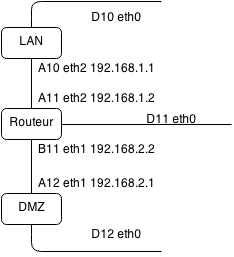
\includegraphics[scale=0.80]{sch1.png}
		\caption{Séance}
	\end{subfigure}%
	~
	\begin{subfigure}[b]{0.4\textwidth}
	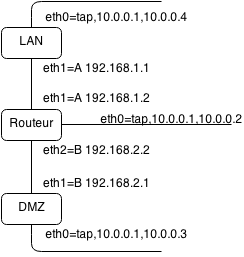
\includegraphics[scale=0.80]{sch2.png}
	\caption{Netkit}
	\label{fig:planadrnetkit}
	\end{subfigure}
	\caption{Plan d'adressage}
\end{figure}

\begin{mdframed}[backgroundcolor=lightred, linecolor=darkred]
Le rapport décrira les différentes étapes du TP en suivant le plan d'adressage de la figure \ref{fig:planadrnetkit} (Netkit).
\end{mdframed}

% après câblage ping possibles: lan <-> routeur et dmz <-> routeur
% il faut activer le routage IP sur le routeur

\newpage

\section{Routage classique}
Nous avons tout d'abord configuré les interfaces Ethernet des 3 machines, ajouté les passerelles par défaut pour LAN et DMZ, et activé le routage IP (IP forwarding) pour le routeur. Le routage IP permet de prendre des décisions concernant le chemin qu'un paquet doit prendre entre les différents réseaux.

\subsection{Configuration du PC Routeur}
\begin{lstlisting}
Router/*:~#*/ echo "1" > /proc/sys/net/ipv4/ip_forward
Router/*:~#*/ ifconfig eth1 192.168.1.2 netmask 255.255.255.0 up
Router/*:~#*/ ifconfig eth2 192.168.2.2 netmask 255.255.255.0 up

Router/*:~#*/ ifconfig
eth0      Link encap:Ethernet  HWaddr 76:f5:98:50:22:50
          inet addr:10.0.0.2  Bcast:10.255.255.255  Mask:255.0.0.0
          ...

eth1      Link encap:Ethernet  HWaddr 7e:a1:77:92:58:e8
          inet addr:192.168.1.2  Bcast:192.168.1.255  Mask:255.255.255.0
          ...

eth2      Link encap:Ethernet  HWaddr 0e:bd:8c:c5:14:02
          inet addr:192.168.2.2  Bcast:192.168.2.255  Mask:255.255.255.0
          ...

/*Router:~#*/ route -n
Kernel IP routing table
Destination     Gateway         Genmask         Flags Metric Ref    Use Iface
192.168.2.0     0.0.0.0         255.255.255.0   U     0      0        0 eth2
192.168.1.0     0.0.0.0         255.255.255.0   U     0      0        0 eth1
10.0.0.0        0.0.0.0         255.0.0.0       U     0      0        0 eth0
0.0.0.0         10.0.0.1        0.0.0.0         UG    0      0        0 eth0
\end{lstlisting}
\hfill

\begin{leftbar}
\noindent Q1. Le répertoire \textbf{/proc/sys} contient des fichiers et sous-répertoires permettant d'activer ou désactiver immédiatement des fonctionnalités du kernel. Le répertoire \textbf{/proc/sys/net} concerne des fonctionnalités réseau, et \textbf{/proc/sys/net/ipv4} concerne plus particulièrement les fonctionnalités liées au protocole IPv4. Par exemple, le fichier \textbf{/proc/sys/net/ipv4/ip\_forward} permet d'activer le routage. Le fichier \textbf{/proc/sys/net/ipv4/icmp\_echo\_ignore\_all} permet d'ignorer les requêtes ECHO du protocole ICMP, ainsi la commande \emph{ping} utilisant ce protocole voit ses requêtes ignorées par une machine ayant \emph{icmp\_echo\_ignore\_all} activé.
% TODO serveurs actifs netstat
\end{leftbar}

\subsection{Configuration du PC LAN}
\begin{lstlisting}
LAN/*:~#*/ ifconfig eth0 down
LAN/*:~#*/ ifconfig eth1 192.168.1.1 netmask 255.255.255.0 up
LAN/*:~#*/ route add default gw 192.168.1.2 eth1

LAN/*:~#*/ ifconfig
eth1      Link encap:Ethernet  HWaddr 42:a7:57:d3:a5:1b
          inet addr:192.168.1.1  Bcast:192.168.1.255  Mask:255.255.255.0
          ...

/*LAN:~#*/ route
Kernel IP routing table
Destination     Gateway         Genmask         Flags Metric Ref    Use Iface
192.168.1.0     *               255.255.255.0   U     0      0        0 eth1
default         192.168.1.2     0.0.0.0         UG    0      0        0 eth1

/*LAN:~#*/ route -n
Kernel IP routing table
Destination     Gateway         Genmask         Flags Metric Ref    Use Iface
192.168.1.0     0.0.0.0         255.255.255.0   U     0      0        0 eth1
0.0.0.0         192.168.1.2     0.0.0.0         UG    0      0        0 eth1
\end{lstlisting}

\subsection{Configuration du PC DMZ}
\begin{lstlisting}
DMZ/*:~#*/ ifconfig eth0 down
DMZ/*:~#*/ ifconfig eth1 192.168.2.1 netmask 255.255.255.0 up
DMZ/*:~#*/ route add default gw 192.168.2.2 eth1

DMZ/*:~#*/ ifconfig
eth1      Link encap:Ethernet  HWaddr 86:e8:ec:bc:60:67
          inet addr:192.168.2.1  Bcast:192.168.2.255  Mask:255.255.255.0
          ...
\end{lstlisting}
\newpage

\subsection{Tables de routage}
\begin{leftbar}
	\noindent Q2. La commande \emph{route -n} permet d'afficher la table de routage IP en remplaçant les noms d'hôtes (provenant par exemple du fichier /etc/hosts) par des adresses numériques. Le symbole * est remplacé par \emph{0.0.0.0}, ce qui désigne la route par défaut. Les tables de routage sur les machines LAN, DMZ et Routeur sont les suivantes :
	\begin{lstlisting}[caption=Table de routage LAN, numbers=none]
Kernel IP routing table
Destination     Gateway         Genmask         Flags Metric Ref    Use Iface
192.168.1.0     0.0.0.0         255.255.255.0   U     0      0        0 eth1
0.0.0.0         192.168.1.2     0.0.0.0         UG    0      0        0 eth1
	\end{lstlisting}
	\begin{lstlisting}[caption=Table de routage DMZ, numbers=none]
Kernel IP routing table
Destination     Gateway         Genmask         Flags Metric Ref    Use Iface
192.168.2.0     0.0.0.0         255.255.255.0   U     0      0        0 eth1
0.0.0.0         192.168.2.2     0.0.0.0         UG    0      0        0 eth1
	\end{lstlisting}
	\begin{lstlisting}[caption=Table de routage Routeur, numbers=none]
Kernel IP routing table
Destination     Gateway         Genmask         Flags Metric Ref    Use Iface
192.168.2.0     0.0.0.0         255.255.255.0   U     0      0        0 eth2
192.168.1.0     0.0.0.0         255.255.255.0   U     0      0        0 eth1
10.0.0.0        0.0.0.0         255.0.0.0       U     0      0        0 eth0
0.0.0.0         10.0.0.1        0.0.0.0         UG    0      0        0 eth0
	\end{lstlisting}
\end{leftbar}

\noindent Suite aux configurations effectuées précédemment, il est possible d'effectuer des pings entre les 3 machines.

\subsection{Configuration du serveur web sur le PC DMZ}
Nous souhaitons ensuite modifier la configuration du serveur http Apache (httpd) pour remplacer le port d'écoute par défaut 80 par le port 8080. Pour cela nous avons modifié le fichier suivant.
\begin{lstlisting}[caption=/etc/httpd/conf/httpd.conf]
Listen 8080
\end{lstlisting}
\hfill

\noindent \textbf{N.B.} Sous une machine (Debian testing) créée à l'aide de netkit utilisant le package apache2 et une configuration par défaut, nous avons dû modifier les fichiers \textbf{/etc/apache2/ports.conf} et \textbf{/etc/apache2/sites-enabled/000-default}. Le premier fichier nous a permis de remplacer le port d'écoute par défaut, le second de modifier le port du VirtualHost (les serveurs virtuels permettent de faire fonctionner plusieurs serveurs web sur une même machine, ici nous n'avons qu'un seul VirtualHost que nous souhaitons associer au port 8080).

\begin{lstlisting}[caption=/etc/apache2/ports.conf, escapechar=@]
# If you just change the port or add more ports here, you will likely also
# have to change the VirtualHost statement in
# /etc/apache2/sites-enabled/000-default
# This is also true if you have upgraded from before 2.2.9-3 (i.e. from
# Debian etch). See /usr/share/doc/apache2.2-common/NEWS.Debian.gz and
# README.Debian.gz

@\textbf{NameVirtualHost *:8080}@
@\textbf{Listen 8080}@

<IfModule mod_ssl.c>
    # SSL name based virtual hosts are not yet supported, therefore no
    # NameVirtualHost statement here
    Listen 443
</IfModule>
\end{lstlisting}

\begin{lstlisting}[caption=/etc/apache2/sites-enabled/000-default, escapechar=\%]
%\textbf{<VirtualHost *:8080>}%
        ServerAdmin webmaster@localhost

        DocumentRoot /var/www/
        <Directory />
                Options FollowSymLinks
                AllowOverride None
        </Directory>
		...
\end{lstlisting}

\noindent Une fois les fichiers de configuration modifiés, il faut relancer le serveur web :
\begin{lstlisting}
/etc/init.d/httpd restart

OU (en fonction de la distribution)

/etc/init.d/apache2 restart
\end{lstlisting}
\hfill

\noindent On peut ensuite vérifier à l'aide de la commande \emph{ps} que le serveur est bien lancé :
\begin{lstlisting}
DMZ/*:~#*/ ps aux | grep apache
root      1010  0.0  8.4  13136  2736 ?        Ss   20:47   0:00 /usr/sbin/apache2 -k start
www-data  1011  0.0  5.9  12908  1928 ?        S    20:47   0:00 /usr/sbin/apache2 -k start
www-data  1013  0.0 10.3 234696  3352 ?        Sl   20:47   0:00 /usr/sbin/apache2 -k start
www-data  1018  0.0 10.3 234696  3340 ?        Sl   20:47   0:00 /usr/sbin/apache2 -k start
root      1116  0.0  2.1   3476   680 tty0     S+   23:45   0:00 grep --color apache
\end{lstlisting}
\hfill

Ci-dessous deux captures d'écran (figures \ref{fig:sch3lan} et \ref{fig:sch3dmz}) de la machine LAN accédant à \textbf{192.168.2.1} (DMZ) sur le port 8080 avec le navigateur web Lynx, et de la machine DMZ observant les paquets reçus sur son interface eth1. Le routeur achemine les paquets de la machine LAN vers la machine DMZ (192.168.1.1:59904 > 192.168.2.1:8080), puis la machine DMZ répond aux requêtes de la machine LAN en envoyant les paquets sur l'interface du routeur à laquelle elle est connectée (192.168.2.1:8080 > 192.168.1.1:59904).

\begin{figure}[h!]
	\centering
	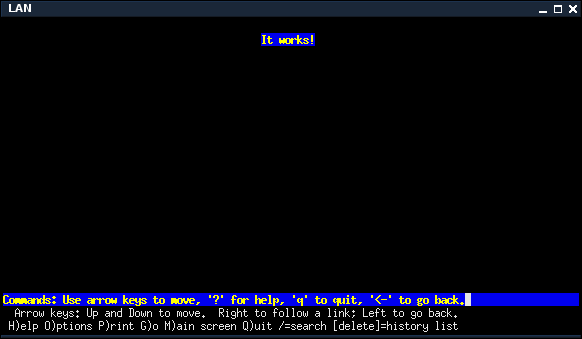
\includegraphics[scale=0.62]{sch3LAN.png}
	\caption{Accès au serveur web (DMZ) depuis Lynx (LAN)}
	\label{fig:sch3lan}
\end{figure}
\newpage

\begin{figure}[h!]
	\centering
	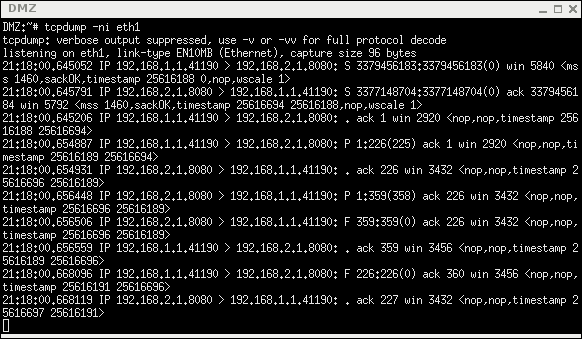
\includegraphics[scale=0.68]{sch3DMZ.png}
	\caption{Paquets reçus par le serveur web (DMZ)}
	\label{fig:sch3dmz}
\end{figure}
\newpage

\section{Mise en oeuvre de la plate-forme sécurisée}
Dans cette partie, nous allons établir des règles de filtrage (table \textbf{filter}) et de translation d'adresse (table \textbf{nat}) à l'aide d'iptables sur le routeur. Pour cela, nous avons créé un script firewall (\emph{/root/firewall}) contenant ces règles.

\begin{leftbar}
	\noindent Q3. Nous souhaitons tout d'abord supprimer les règles établies précédemment, puis rejeter par défaut tous les paquets (INPUT, OUTPUT et FORWARD). Nous établirons par la suite des règles permettant d'autoriser des paquets répondant à certains critères.
	\begin{lstlisting}[numbers=none]
# Flush filter and nat tables
iptables -F
iptables -F -t nat

# Policy : drop all
iptables -P INPUT DROP
iptables -P OUTPUT DROP
iptables -P FORWARD DROP
	\end{lstlisting}
\end{leftbar}

La politique par défaut pour les 3 chaînes (INPUT, OUTPUT, FORWARD) est de rejeter les paquets, il n'est donc entre autres plus possible de ping les 3 PCs entre eux.

\begin{leftbar}
	\noindent Q4. Après exécution du script, les règles d'iptables peuvent être observées à l'aide de la commande \emph{iptables -L}. Nous pouvons observer que la politique par défaut est effectivement le rejet de paquet pour chaque chaîne (e.g. \emph{Chain INPUT (policy DROP)}).
	\begin{lstlisting}[numbers=none]
Router/*:~#*/ iptables -L
Chain INPUT (policy DROP)
target     prot opt source               destination

Chain FORWARD (policy DROP)
target     prot opt source               destination

Chain OUTPUT (policy DROP)
target     prot opt source               destination
	\end{lstlisting}
\end{leftbar}

\subsection{Filtrage entre LAN et DMZ}
Nous souhaitons cacher l'existence des machines du réseau LAN aux machines de la DMZ. Avant cela, nous allons établir des règles dans le firewall pour autoriser certains paquets.

\begin{leftbar}
	\noindent Q5. Nous allons tout d'abord autoriser le réseau LAN à envoyer des requêtes du protocole ICMP, puis le routeur à répndre à ces requêtes. Cela va permettre d'accepter un ping venant du réseau LAN (\textbf{192.168.1.0/24}) adressé à l'interface du routeur côté LAN (\textbf{192.168.1.2}).
	\begin{lstlisting}[numbers=none]
# accept ping LAN -> routeur
iptables -A INPUT -s 192.168.1.0/24 -d 192.168.1.2 -p icmp --icmp-type echo-request -j ACCEPT
iptables -A OUTPUT -s 192.168.1.2 -d 192.168.1.0/24 -p icmp --icmp-type echo-reply -j ACCEPT
	\end{lstlisting}
	\hfill

	\noindent Une alternative possible est d'autoriser les requêtes du protocole ICMP provenant du réseau LAN (\textbf{192.168.1.0/24}) adressées à l'interface \textbf{eth1} du routeur (reliée au réseau LAN), puis d'autoriser les réponses du protocole ICMP sortant du routeur par l'interface \textbf{eth1} en direction du réseau LAN.
	\begin{lstlisting}[numbers=none]
# alternative
iptables -A INPUT -s 192.168.1.0/24 -i eth1 -p icmp --icmp-type echo-request -j ACCEPT
iptables -A OUTPUT -o eth1 -d 192.168.1.0/24 -p icmp --icmp-type echo-reply -j ACCEPT
	\end{lstlisting}
	\hfill

	\noindent Une autre alternative possible pour la sortie du routeur est d'autoriser les paquets du protocole ICMP ayant déjà une connexion établie. Nous pouvons aussi par exemple retirer les options -s et/ou -d pour réduire les conditions devant être remplies pour qu'une réponse soit acceptée.
	\begin{lstlisting}[numbers=none]
iptables -A OUTPUT -s 192.168.1.2 -d 192.168.1.0/24 -p icmp -m state --state ESTABLISHED,RELATED -j ACCEPT
	\end{lstlisting}
\end{leftbar}

\begin{leftbar}
	\noindent Q6. De manière similaire, nous autorisons le réseau DMZ (\textbf{192.168.2.0/24}) à envoyer des ping à l'interface du routeur côté DMZ (\textbf{192.168.2.2}), puis au routeur d'envoyer une réponse à ces requêtes.
	\begin{lstlisting}[numbers=none]
# accept ping DMZ -> routeur
iptables -A INPUT -s 192.168.2.0/24 -d 192.168.2.2 -p icmp --icmp-type echo-request -j ACCEPT
iptables -A OUTPUT -s 192.168.2.2 -d 192.168.2.0/24 -p icmp --icmp-type echo-reply -j ACCEPT
	\end{lstlisting}
\end{leftbar}

\begin{leftbar}
	\noindent Q7. Enfin, à l'aide de règles FORWARD, nous souhaitons que le routeur laisse passer les requêtes du protocole ICMP provenant du réseau LAN (\textbf{192.168.1.0/24}) à destination du réseau DMZ (\textbf{192.168.2.0/24}), et les réponses du réseau DMZ à destination du réseau LAN.
	\begin{lstlisting}[numbers=none]
# accept ping LAN -> DMZ
iptables -A FORWARD -s 192.168.1.0/24 -d 192.168.2.0/24 -p icmp --icmp-type echo-request -j ACCEPT
iptables -A FORWARD -s 192.168.2.0/24 -d 192.168.1.0/24 -p icmp --icmp-type echo-reply -j ACCEPT
	\end{lstlisting}
\end{leftbar}

Le PC LAN peut à présent envoyer un ping à destination du PC DMZ. Ci-dessous l'exécution d'un ping de LAN vers DMZ et un tcpdump sur la machine DMZ.
\begin{lstlisting}
LAN/*:~#*/ ping 192.168.2.1
PING 192.168.2.1 (192.168.2.1) 56(84) bytes of data.
64 bytes from 192.168.2.1: icmp_seq=1 ttl=63 time=0.245 ms
64 bytes from 192.168.2.1: icmp_seq=2 ttl=63 time=0.271 ms
64 bytes from 192.168.2.1: icmp_seq=3 ttl=63 time=0.630 ms
...
-----------------------------------------------------------------------------------------------
DMZ/*:~#*/ tcpdump -ni eth1
tcpdump: verbose output suppressed, use -v or -vv for full protocol decode
listening on eth1, link-type EN10MB (Ethernet), capture size 96 bytes
07:34:05.156294 IP 192.168.1.1 > 192.168.2.1: ICMP echo request, id 22530, seq 1, length 64
07:34:05.156838 IP 192.168.2.1 > 192.168.1.1: ICMP echo reply, id 22530, seq 1, length 64
07:34:06.155243 IP 192.168.1.1 > 192.168.2.1: ICMP echo request, id 22530, seq 2, length 64
07:34:06.155262 IP 192.168.2.1 > 192.168.1.1: ICMP echo reply, id 22530, seq 2, length 64
07:34:07.155179 IP 192.168.1.1 > 192.168.2.1: ICMP echo request, id 22530, seq 3, length 64
07:34:07.155250 IP 192.168.2.1 > 192.168.1.1: ICMP echo reply, id 22530, seq 3, length 64
...
\end{lstlisting}
Le \emph{tcpdump} nous permet d'observer que des paquets de la machine LAN (\textbf{192.168.1.1}) correspondant à des requêtes ICMP (ICMP echo request) sont reçues par la machine DMZ (\textbf{192.168.2.1}), puis que des réponses ICMP (ICMP echo reply) sont envoyées de la machine DMZ vers la machine LAN. L'option \emph{-n} permet de ne pas convertir les adresses, c'est à dire de conserver des adresses numériques.\\

\begin{leftbar}
	\noindent Q8. Nous souhaitons à présent à l'aide de la table nat d'\emph{iptables} faire la translation d'adresses du ping du réseau LAN vers la DMZ afin de masquer l'existence du réseau LAN à la DMZ.
	\begin{lstlisting}[numbers=none]
# translation d'adresse ping LAN -> DMZ
iptables -t nat -A POSTROUTING -s 192.168.1.0/24 -d 192.168.2.0/24 -j SNAT --to-source 192.168.2.2 -p icmp --icmp-type echo-request
	\end{lstlisting}
	La chaîne POSTROUTING associée à la cible SNAT permet de masquer l'émetteur d'un paquet par l'IP précisée par l'option \emph{-\--to-source}. Ci-dessous un ping du PC LAN (\textbf{192.168.1.1}) vers le PC DMZ (\textbf{192.168.2.1}), et un tcpdump effectué sur le PC DMZ.
	\begin{lstlisting}[numbers=none]
LAN/*:~#*/ ping 192.168.2.1
PING 192.168.2.1 (192.168.2.1) 56(84) bytes of data.
64 bytes from 192.168.2.1: icmp_seq=1 ttl=63 time=19.2 ms
64 bytes from 192.168.2.1: icmp_seq=2 ttl=63 time=0.613 ms
64 bytes from 192.168.2.1: icmp_seq=3 ttl=63 time=0.514 m
...
-----------------------------------------------------------------------------------------------
Router/*:~#*/ iptables -L -t nat
Chain PREROUTING (policy ACCEPT)
target     prot opt source               destination

Chain POSTROUTING (policy ACCEPT)
target     prot opt source               destination
SNAT       icmp --  192.168.1.0/24       192.168.2.0/24      icmp echo-request to:192.168.2.2

Chain OUTPUT (policy ACCEPT)
target     prot opt source               destination
-----------------------------------------------------------------------------------------------
DMZ/*:~#*/ tcpdump -ni eth1
tcpdump: verbose output suppressed, use -v or -vv for full protocol decode
listening on eth1, link-type EN10MB (Ethernet), capture size 96 bytes
07:49:06.399986 arp who-has 192.168.2.1 tell 192.168.2.2
07:49:06.400679 arp reply 192.168.2.1 is-at 86:e8:ec:bc:60:67
07:49:06.400021 IP 192.168.2.2 > 192.168.2.1: ICMP echo request, id 22786, seq 1, length 64
07:49:06.400060 IP 192.168.2.1 > 192.168.2.2: ICMP echo reply, id 22786, seq 1, length 64
07:49:07.405204 IP 192.168.2.2 > 192.168.2.1: ICMP echo request, id 22786, seq 2, length 64
07:49:07.405254 IP 192.168.2.1 > 192.168.2.2: ICMP echo reply, id 22786, seq 2, length 64
07:49:08.415065 IP 192.168.2.2 > 192.168.2.1: ICMP echo request, id 22786, seq 3, length 64
07:49:08.415141 IP 192.168.2.1 > 192.168.2.2: ICMP echo reply, id 22786, seq 3, length 64
...
	\end{lstlisting}
	Nous pouvons observer sur le \emph{tcpdump} ci-dessus que la source du paquet (initialement \textbf{192.168.1.1}) a été masquée et modifiée par l'IP de l'interface du routeur côté DMZ (\textbf{192.168.2.2}).
\end{leftbar}
\hfill

Nous avons autorisé le ping de LAN vers DMZ puis masqué l'IP source des paquets provenant de LAN adressés à DMZ, nous souhaitons à présent faire de même pour l'accès au serveur http depuis le PC LAN.

\begin{leftbar}
	\noindent Q9. A l'aide de règles FORWARD, nous autorisons les requêtes du protocole TCP sur le port 8080 provenant du réseau LAN (\textbf{192.168.1.0/24}) et adressées au PC DMZ (\textbf{192.168.2.1}), puis les réponses du PC DMZ vers le réseau LAN pour les connexions déjà établies.
	\begin{lstlisting}[numbers=none]
# accept LAN -> serveur http DMZ (port 8080)
iptables -A FORWARD -s 192.168.1.0/24 -d 192.168.2.1 -p tcp --dport 8080 -j ACCEPT
iptables -A FORWARD -s 192.168.2.1 -d 192.168.1.0/24 -p tcp -m state --state ESTABLISHED,RELATED -j ACCEPT
	\end{lstlisting}
	Nous ajoutons ensuite une règle dans la table nat d'iptables permettant de masquer l'IP des machines du réseau LAN par l'IP de l'interface du routeur côté DMZ.
	\begin{lstlisting}[numbers=none]
# translation d'adresse LAN -> serveur http DMZ
iptables -t nat -A POSTROUTING -s 192.168.1.0/24 -d 192.168.2.1 -j SNAT --to-source 192.168.2.2 -p tcp
	\end{lstlisting}
	Ci-dessous le \emph{tcpdump} effectué sur la machine DMZ pour un accès au serveur http depuis le PC LAN:
	\begin{lstlisting}[numbers=none]
LAN/*:~#*/ lynx 192.168.2.1:8080
-----------------------------------------------------------------------------------------------
DMZ/*:~#*/ tcpdump -ni eth1
tcpdump: verbose output suppressed, use -v or -vv for full protocol decode
listening on eth1, link-type EN10MB (Ethernet), capture size 96 bytes
08:27:05.666691 IP 192.168.2.2.43830 > 192.168.2.1.8080: S 1997685473:1997685473(0) win 5840 <mss 1460,sackOK,timestamp 38270691 0,nop,wscale 1>
08:27:05.667630 IP 192.168.2.1.8080 > 192.168.2.2.43830: S 2000354492:2000354492(0) ack 1997685474 win 5792 <mss 1460,sackOK,timestamp 38271196 38270691,nop,wscale 1>
08:27:05.666860 IP 192.168.2.2.43830 > 192.168.2.1.8080: . ack 1 win 2920 <nop,nop,timestamp 38270691 38271196>
08:27:05.667287 IP 192.168.2.2.43830 > 192.168.2.1.8080: P 1:226(225) ack 1 win 2920 <nop,nop,timestamp 38270691 38271196>
08:27:05.667311 IP 192.168.2.1.8080 > 192.168.2.2.43830: . ack 226 win 3432 <nop,nop,timestamp 38271196 38270691>
08:27:05.669430 IP 192.168.2.1.8080 > 192.168.2.2.43830: P 1:359(358) ack 226 win 3432 <nop,nop,timestamp 38271196 38270691>
08:27:05.669548 IP 192.168.2.1.8080 > 192.168.2.2.43830: F 359:359(0) ack 226 win 3432 <nop,nop,timestamp 38271196 38270691>
08:27:05.669614 IP 192.168.2.2.43830 > 192.168.2.1.8080: . ack 359 win 3456 <nop,nop,timestamp 38270691 38271196>
08:27:05.670869 IP 192.168.2.2.43830 > 192.168.2.1.8080: F 226:226(0) ack 360 win 3456 <nop,nop,timestamp 38270691 38271196>
08:27:05.670888 IP 192.168.2.1.8080 > 192.168.2.2.43830: . ack 227 win 3432 <nop,nop,timestamp 38271196 38270691>

	\end{lstlisting}
\end{leftbar}

Les deux règles de translation d'adresse définies précédemment peuvent être remplacées par une règle plus générale. Nous pouvons en effet masquer l'IP des paquets du réseau LAN adressés au réseau DMZ pour tous les protocoles.
\begin{lstlisting}
iptables -t nat -A POSTROUTING -s 192.168.1.0/24 -d 192.168.2.0/24 -j SNAT --to-source 192.168.2.2
\end{lstlisting}

\subsection{Filtrage LAN et Internet}
Les machines du réseau LAN ne doivent pas être directement visibles d'Internet. Nous devons donc tout d'abord désactiver l'interface \textbf{eth0} sur le PC LAN pour ne plus avoir d'accès direct à Internet (déjà effectué précédemment).
\begin{lstlisting}
LAN/*:~#*/ ifconfig eth0 down
\end{lstlisting}

\begin{leftbar}
	\noindent Q10.
	Pour que les machines du réseau local (LAN, \textbf{192.168.1.0/24}) puissent communiquer avec des machines du réseau Internet (interface \textbf{eth0} du routeur) en passant par le routeur, il faut tout d'abord ajouter une règle IP Masquerade dans la table nat d'\emph{iptables} sur le routeur. IP Masquerade est un type de translation d'adresse permettant de remplacer l'IP des paquets du réseau local par l'IP du routeur côté Internet. Cela permet donc à un réseau local d'accéder à Internet avec une seule IP.
	\begin{lstlisting}[numbers=none]
# IP Masquerade
iptables -t nat -A POSTROUTING -s 192.168.1.0/24 -o eth0 -j MASQUERADE
	\end{lstlisting}
	On autorise ensuite le réseau LAN à ping (protocole ICMP) une machine sur le réseau Internet en passant par le routeur.
	\begin{lstlisting}[numbers=none]
# ping LAN -> Internet
iptables -A FORWARD -s 192.168.1.0/24 -o eth0 -p icmp --icmp-type echo-request -j ACCEPT
iptables -A FORWARD -i eth0 -d 192.168.1.0/24 -m state --state ESTABLISHED,RELATED -p icmp -j ACCEPT
	\end{lstlisting}
	De même pour le protocole HTTP (couche application), nous autorisons le réseau LAN à envoyer des requêtes du protocole TCP (couche transport) sur les ports 80 (port par défaut HTTP) et 443 (port par défaut HTTPS) vers le port eth0 du routeur, et le routeur à répondre pour des connexions déjà établies.
	\begin{lstlisting}[numbers=none]
iptables -A FORWARD -s 192.168.1.0/24 -o eth0 -p tcp -m multiport --dports 80,443 -j ACCEPT
iptables -A FORWARD -i eth0 -d 192.168.1.0/24 -p tcp -m state --state ESTABLISHED,RELATED -j ACCEPT
	\end{lstlisting}
\end{leftbar}

\begin{leftbar}
	\noindent Q11. Pour pouvoir utiliser les noms de domaines, il faut que les serveurs DNS puissent être joignables. Ces \emph{name servers} sont définis dans le fichier \textbf{/etc/resolv.conf}.
	\begin{lstlisting}[caption=Exemple de nameservers (Google Public DNS) dans /etc/resolv.conf, numbers=none]
nameserver 8.8.8.8
nameserver 8.8.4.4
	\end{lstlisting}
	DNS utilise le protocole UDP sur le port 53, il faut donc autoriser ces requêtes provenant de LAN vers Internet, puis les réponses pour les connexions déjà établies dans le sens inverse.
	\begin{lstlisting}[numbers=none]
# LAN -> DNS
iptables -A FORWARD -s 192.168.1.0/24 -o eth0 -p udp --dport 53 -j ACCEPT
iptables -A FORWARD -i eth0 -d 192.168.1.0/24 -p udp -m state --state ESTABLISHED,RELATED -j ACCEPT
	\end{lstlisting}
\end{leftbar}

\subsection{Filtrage DMZ et Internet}
Le PC DMZ ne doit pas être directement visible d'Internet, nous devons donc désactiver son interface eth0 (déjà effectué précédemment).
\begin{lstlisting}
DMZ/*:~#*/ ifconfig eth0 down
\end{lstlisting}
De plus, nous allons utiliser le PC LAN pour simuler un accès d'une machine Internet. Nous devons donc réactiver son interface eth0 et désactiver son interface eth1. Sous Netkit, nous devons également ajouter la passerelle par défaut pour eth0 ayant pour IP celle de l'interface ajoutée sur le PC hôte.
\begin{lstlisting}
LAN/*:~#*/ ifconfig eth1 down
LAN/*:~#*/ ifconfig eth0 up
LAN/*:~#*/ route add default gw 10.0.0.1 eth0
LAN/*:~#*/ route -n
Kernel IP routing table
Destination     Gateway         Genmask         Flags Metric Ref    Use Iface
10.0.0.0        0.0.0.0         255.0.0.0       U     0      0        0 eth0
0.0.0.0         10.0.0.1        0.0.0.0         UG    0      0        0 eth0
\end{lstlisting}

\begin{leftbar}
	\noindent Q12. Les requêtes envoyées sur l'adresse IP associée à l'interface eth0 du routeur (\textbf{10.0.0.2} ) sur le port 80 doivent être redirigées sur la DMZ (\textbf{192.168.2.1}) sur le port 8080. Pour cela nous ajoutons une règle PREROUTING dans la table nat d'iptables, permettant ainsi de masquer la destination du paquet, et de la remplacer par \textbf{192.168.2.1:8080}. Nous devons également autoriser les paquets du protocole TCP passant par le routeur entrant par l'interface eth0 à destination du PC DMZ sur le port 8080, et les réponses en sens inverse pour les connexions déjà établies.
	\begin{lstlisting}[numbers=none]
# 3.3 Filtrage DMZ et Internet
iptables -t nat -A PREROUTING -i eth0 -d 10.0.0.2 -p tcp --dport 80 -j DNAT --to-destination 192.168.2.1:8080
iptables -A FORWARD -i eth0 -d 192.168.2.1 -p tcp --dport 8080 -j ACCEPT
iptables -A FORWARD -s 192.168.2.1 -o eth0 -p tcp --sport 8080 -m state --state ESTABLISHED,RELATED -j ACCEPT
	\end{lstlisting}
\end{leftbar}

\begin{leftbar}
	\noindent Q13. L'option \emph{-w} de \emph{tcpdump} permet d'écrire les paquets reçus dans un fichier, et l'option \emph{-s 0} permet de ne pas tronquer les paquets.
	\begin{lstlisting}[numbers=none]
LAN/*:~#*/ lynx 10.0.0.2
-----------------------------------------------------------------------------------------------
DMZ/*:~#*/ tcpdump -ni eth1 -s 0 -w /hosthome/Documents/dump2.pcap
tcpdump: listening on eth1, link-type EN10MB (Ethernet), capture size 65535 bytes
^C12 packets captured
12 packets received by filter
0 packets dropped by kerne
	\end{lstlisting}
	Le fichier peut être ensuite analysé à l'aide de \emph{wireshark} (figure \ref{fig:wireshark}). Wireshark permet de visualiser pour chaque paquet les en-têtes ajoutés par les différents protocoles, ainsi que les données. Sur la figure \ref{fig:wireshark}, nous pouvons observer deux paquets ayant la couche réseau comme couche la plus élevée et utilisant le protocole ARP permettant de traduire une IP en adresse physique (adresse Ethernet ici). Nous pouvons également observer une requête provenant du protocole HTTP (GET / HTTP.1.0) et la réponse associée :
	\begin{lstlisting}[numbers=none]
Line-based text data: text/html
	<html><body><h1>It works!</h1></body></html>\n
	\end{lstlisting}
\end{leftbar}

\begin{figure}[h!]
	\centering
	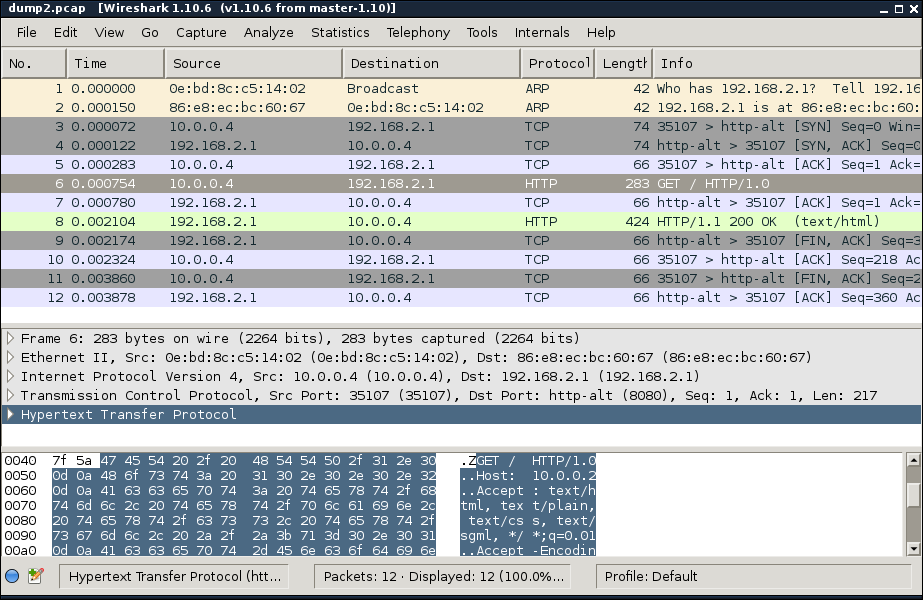
\includegraphics[scale=0.55]{wireshark.png}
	\caption{Sortie de tcpdump visualisée avec wireshark}
	\label{fig:wireshark}
\end{figure}
\newpage

\makeatletter
\renewcommand\refname{Ressources utilisées}
\renewcommand\@biblabel[1]{\textbullet}
\makeatother
\begin{thebibliography}{5}
\bibitem{bib:netkitwiki} \emph{Netkit Wiki}, \href{http://wiki.netkit.org/index.php/Main_Page}{http://wiki.netkit.org/index.php/Main\_Page}
\bibitem{bib:netkittuto1} \emph{Dante's Lab: Creating virtual laboratories with Netkit (I)}, \href{http://danteslab-eng.blogspot.fr/2013/10/creating-virtual-laboratories-with.html}{http://danteslab-eng.blogspot.fr/2013/10/ creating-virtual-laboratories-with.html}
\bibitem{bib:netkittuto2} \emph{Dante's Lab: Creating virtual laboratories with Netkit (II)}, \href{http://danteslab-eng.blogspot.fr/2013/10/creating-virtual-laboratories-with_19.html}{http://danteslab-eng.blogspot.fr/2013/10/ creating-virtual-laboratories-with\_19.html}
\end{thebibliography}

\end{document}
